
%%%%%%%%%%%%%%%%%%%%%%%%%%%%%%%%%%%%%%%%%%%%%%%%%%%%%%%%%%


% Coordinates at Intersections in TikZ: Newton’s Method Case
% https://latexdraw.com
% 05/07/2020, 20:53


\documentclass[border=0.5cm]{standalone}

\usepackage{tikz}
\usetikzlibrary{intersections}

\begin{document}

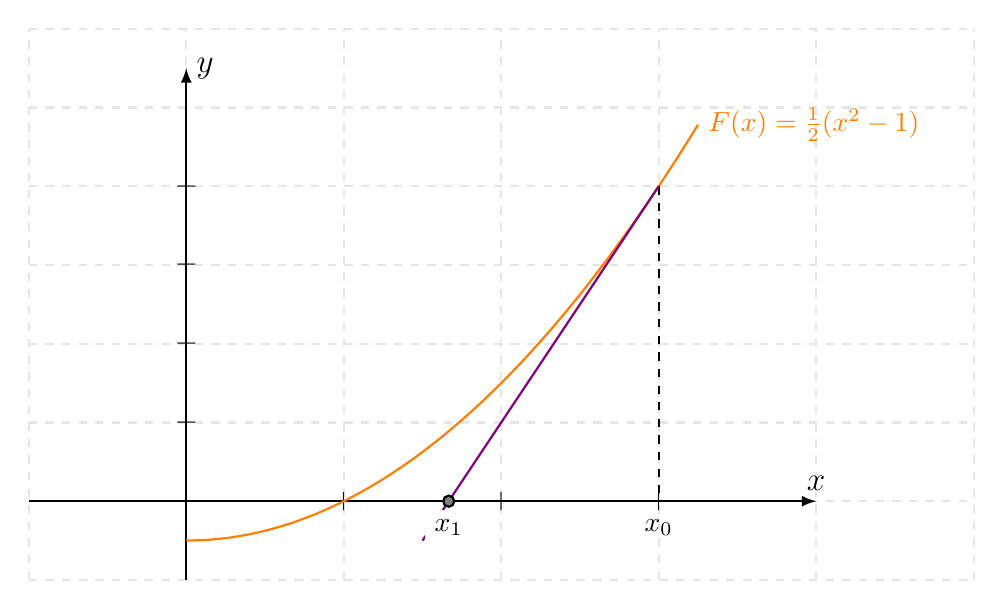
\begin{tikzpicture}[thick,x=2cm]

% Axes
\draw[black!10,dashed,xstep=2cm] (-1,-1) grid(5,6);
\draw[-latex,name path=xaxis] (-1,0) -- (4,0) node[above]{\large $x$};
\draw[-latex] (0,-1) -- (0,5.5)node[right]{\large $y$};
\foreach \i in {1,2,3} {\node at (\i,0) {$+$};}
\foreach \i in {1,2,3,4} {\node at (0,\i) {$+$};}

% Function plot
\draw[orange,name path=Fx]  plot[smooth,domain=0:3.25] (\x, {0.5*\x^2-0.5}) 
node[right](Fx){$F(x)=\frac{1}{2}(x^2-1)$};

% Dashed line
\draw [dashed] (3,4) -- (3,0) 
node[below=0.1cm] {$x_{0}$} ;

% plot tangent line
\draw[violet,name path=Tangent] plot[smooth,domain=1.5:3] (\x, {3*\x-5});

%  Intersection
\draw [name intersections={of=Tangent and xaxis},fill=gray]
(intersection-1) circle(2pt) 
node[below=0.1cm,fill=white]{$x_{1}$} ;

\end{tikzpicture}

\end{document}